%~ \documentclass[10pt]{article} % 11 Arial

% \usepackage{fontspec}
% \setmainfont{Arial}
%~ \usepackage{setspace}
% \onehalfspacing
% \usepackage[english]{babel}
% \usepackage{natbib}
%~ \usepackage{url}
%~ \usepackage[utf8x]{inputenc}
%~ \usepackage{amsmath}
%~ \usepackage{graphicx}

%~ \graphicspath{{images/}}
%~ \usepackage{parskip}
%~ \usepackage{fancyhdr}
%~ \usepackage{vmargin}
%~ \setmarginsrb{2 cm}{2 cm}{4 cm}{2 cm}{2 cm}{1.5 cm}{1 cm}{1.5 cm}



%~ \title{}								% Title
%~ \author{ D. Rabizo (1468883)}								% Author


%\makeatletter
%\let\thetitle\@title
%\let\theauthor\@author
%\let\thedate\@date
%\makeatother

%~ \pagestyle{fancy}
%~ \fancyhf{}
%~ \rhead{\theauthor}
%~ \lhead{\thetitle}
%~ \cfoot{\thepage}

%~ \begin{document}

%%%%%%%%%%%%%%%%%%%%%%%%%%%%%%%%%%%%%%%%%%%%%%%%%%%%%%%%%%%%%%%%%%%%%%%%%%%%%%%%%%%%%%%%%



%%%%%%%%%%%%%%%%%%%%%%%%%%%%%%%%%%%%%%%%%%%%%%%%%%%%%%%%%%%%%%%%%%%%%%%%%%%%%%%%%%%%%%%%%

%\tableofcontents
%\pagebreak

%%%%%%%%%%%%%%%%%%%%%%%%%%%%%%%%%%%%%%%%%%%%%%%%%%%%%%%%%%%%%%%%%%%%%%%%%%%%%%%%%%%%%%%%%




\section{Relationale Ära} %here begins the main part


Heutzutage sind relationale Datenbanken eine der wichtigsten Teilen aller modernen Informationssystemen. In dem Gebiet der praktischen Programmierung haben sich neue Technologien, Plattformen der Realisation und Umgebungen rasant entwickelt, nichtsdestotrotz bleibt der klassische anerkannte Ansatz zur Modellierung und Projektierung der relationalen Datenbanken aktuell. Relationen Modell und ihre Grundlagen sind weit verbreitet bei der Erstellung von relationalen Datenbanken. Die Darstellung von Daten in Form von einer Gesamtheit von Tabellen hat es gestattet, dass mehrere Nachteile der früheren Datenbanksystemen vermieden werden, und neue Systeme mit der vereinfachten Interface-basierten Verwaltung erzeugt werden. In der heutigen Zeit ist eine große Anzahl von den Datenbanken-Server auf dem Prinzip von relationalen Datenmodell basiert, deswegen möchten wir das Konzept und Geschichte des relationalen Modells näher betrachten.


Das Relationalle Modell erschien infolge der Arbeit von dem britischen Wissenschaftler Edgar Codd bei IBM, seitdem er im Jahr 1970 einen Artikel «Relational Model of Data for Large Shared Data Banks» veröffentlicht hat. Er ist zum Begründer der modernen Datenbanktechnologie geworden, sodass er dafür im Jahr 1981 den Turing Award ausgezeichnet wurde. Im einleitenden Teil seines Artikels, kritisiert E. Codd hierarchisches Datenbanksystem (IMS) und Netzwerk-Datenbanksystem CODASYL, die nicht eine eindeutige Darstellung von Beziehungen auf der physischen Ebene gewährleisten können \cite{codd1970relational}. 

Auf einem einfachen Beispiel zeigt er, dass das gleiche Datenschema in fünf verschiedenen Arten der physischen Organisation von Einträgen dargestellt werden kann. Es wird dadurch komplizierter, dass es sowohl eine Fülle an Zeiger existieren soll, als auch die Einträge (Segmente) organisiert werden sollen, was wiederum die Abhängigkeit zwischen den Daten verstärkt. Edgar Codd versucht diese Abhängigkeit loszuwerden \cite{stonebraker2005goes} indem er bietet, alle Daten einschließlich die Abhängigkeiten wischen den Objekten in Form von Beziehungen (zweidimensionalen Tabellen) zu speichern. Der Vorteil des relationalen Datenmodells ist seine Deutlichkeit, Klarheit und Einfachheit der physikalischen Implementierung auf einem Computer. Diese Einfachheit und Klarheit waren als Hauptgrund für den Anwender für die weitverbreitete Anwendung. Die Probleme mit der Effizienz von Datenverarbeitung war technisch ziemlich auflösbar. Die Hauptnachteile des relationalen Datenmodells sind unter anderem das Fehlen von Standardmitteln zur Identifizierung einzelnen Datensätzen, Schwierigkeit der Beschreibung der hierarchischen und Netzwerkabhängigkeiten. Das Datenschema besteht aus den einzelnen Tabellen. Jede Spalte dieser Tabellen entspricht einem Attribut (Element in den Netzwerkdatenbanken) und jede Zeile (Tupel) einem Datensatz. Die Reihenfolge der Zeilen kann beliebig sein. Tabellen in dem relationalen Datenmodell haben eine Menge von Eigenschaften. Die wichtigsten sind \cite{sauer2002relationale}: 
\begin{itemize}
\item  Die Tabelle kann keine gleiche Datensätze beinhalten. Alle Tabellen, die diese Bedingung erfüllen heißen Relationen in der Mathematik.
\item Die Spalten der Tabelle haben eine bestimmte Reihenfolge, die bei der Erzeugung von der Tabelle festgelegt wird. Die Tabelle kann auch keinen einzigen Dateneintrag beinhalten, aber  es muss zumindest eine Spalte vorhanden sein.
\item  Jede Spalte hat einen eindeutigen Namen(innerhalb der Tabelle), und alle Einträge müssen einen einzigen Datentyp haben.
\item Jede Spalte hat einen eindeutigen Namen(innerhalb der Tabelle), und alle Einträge müssen einen einzigen Datentyp haben.
\item In der Spalten-Zeilen Kreuzung muss ein atomares Eintrag sein, die nicht aus einer Gruppe von Einträge besteht. Tabelle, die diese Bedingung erfüllen, heißen Normalisiert.
\item Relation ist eine bestimmte Abhängigkeit zwischen den übereinstimmenden Werten in den Tabellen (Schlüssel aus einer Tabelle und Fremdschlüssel aus der anderen). Es gibt mehrere arten von Abhängigkeiten, und zwar 1:1, 1:n und n:m, die wir weiter behandeln.
\end{itemize}

Bei der Verwendung von 1:1 Abhängigkeit kann ein Datensatz in der Tabelle nicht mehr als nur einen verbundenen Datensatz in der Anderen Tabelle haben.Bei der 1:n Verbindung, kann einem Datensatz aus einer Tabelle mehrere Tupel aus der anderen Tabelle entsprechen, wobei jedem Datensatz aus der zweiten Tabelle kann nur ein Datensatz in der ersten entsprechen. Bei der n:m Abhängigkeit können mehrere Datensätze aus der ersten Tabelle den Datensätzen aus den zweiten entsprechen, und umgekehrt. Die n:m Beziehung wird praktisch nicht besonders oft in der relationalen Umgebung realisiert, aber sie lässt sich mit der Einführung von einer zusätzlichen Relation leicht lösen. 
	Eine Menge von Datentypen, die von den relationalen Datenbanksystemen unterstützt werden, umfasst einfache (atomare) Typen, die wir aus den üblichen Programmiersprachen wissen, und zwar: logischer Typ (boolean), numerischer Typ (integer, float), Datum/Zeit sowie ein String Typ. 
	Um das Konzept von Relationen Datenbanken besser zu zu verdeutlichen, haben wir ein einfaches Beispiel mit der Relation «Arbeiter», die eine eindeutig identifizierende Nummer hat, Vor- und Nachnamen, Geburtsdatum, Geschlecht und Dienststelle. Es gibt auch Relation «Abteilung», die einen eindeutigen Namen hat, Stiege, Stock, Raum und Telefonnummer. Mit der Relation «Arbeiter der Abteilung» lässt sich eine n:m Relation darstellen, in der einem Namen der Abteilung wird eine Nummer des Arbeiters zugewiesen. 
 \begin{center} 
 Relation Arbeiter
   


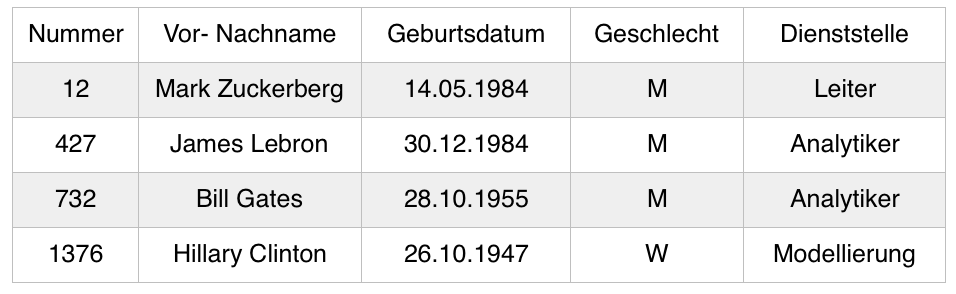
\includegraphics[width=0.7\textwidth]{images/Arbeiter.png}
 
Relation Abteilung 

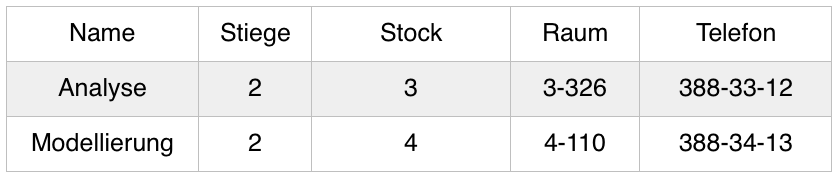
\includegraphics[width=0.7\textwidth]{images/Abteilung.png}

Relation Arbeiter in der Abteilung

 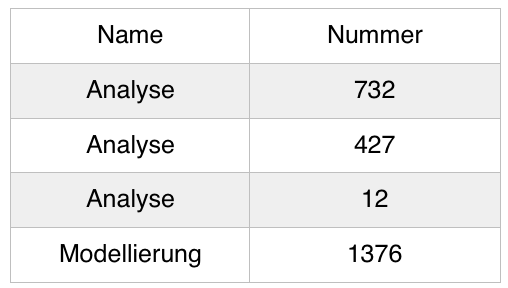
\includegraphics[width=0.4\textwidth]{images/Arbeiter_Abteilung.png} 
 \end{center}
 
 
Bestandteile der Tabellen: 

\textit{\textbf{Schlüsselattribut}} - eine Spalte in der Tabelle, deren Einträge alle unterschiedlich sind, weil ein Schlüsselattribut eindeutig identifizierend sein soll. In der Tabelle «Arbeiter», zum Beispiel, ist Nummer der Schlüsselattribut.

\textit{\textbf{Fremdschlüssel}} - ein Attribut in der Relation, der auf eine Andere Relation verweist, um eine Beziehung zwischen den Tabellen darzustellen.

Zum Beispiel in der Tabelle «Arbeiter der Abteilung» sind Name und Nummer Fremdschlüssel, die entsprechend auf Arbeiter und Abteilungen verweisen. 
Relation-Datenbanksysteme haben zuerst keine große Verbreitung bekommen, da es sehr lange Zeit eine Meinung herrschte, dass es unmöglich wäre, eine effiziente Implementierung solcher Datenbanksystemen zu erreichen, aber die oben beschriebene Vorteile (Einfachheit, Klarheit) und allmähliche Akkumulation der Methoden und Algorithmen zur Organisation und Manipulation von Realtion-Datenbanken haben dazu geführt, dass relationale Datenbanksysteme von dem Weltmarkt alle früher benutze Datenbanken verdrängt haben. Damals im Jahr 1970 hatten die Entwickler erst die Theoretische Aspekte des relationalen Datenbanksystems entworfen, und kurz danach erschienen die erste Prototypen. Das erste Relationale Datenbanksystem war «System R», die in der Mitte von 1970 Jahren, im Rahmen eines Entwicklungsprojektes von IBM entwickelt wurde. Obwohl die Ideen von Edgar Codd für die Entwicklung von System R zugrunde gelegt wurden, hat er persönlich im Projekt nicht teilgenommen. Für die Arbeit mit Daten wurde eine spezifische Sprache erfunden, die SEQUEL hieß (Structed English QUEry Language) und dann im Laufe der Zeit in SQL umbenennt (Structed Query Language) wurde. Bei dem Schaffen von SQL haben die Entwickler von System R haben die Theorie eines relationalen Modelles ziemlich frei formuliert. Codd hat Ihm zusammen mit dem Programmierer Christopher J. Date verlassen, und ein unabhängiges Beratungsunternehmen gegründet, in dem sie ihre Arbeit mit dem relationalen Modell fortgesetzt haben. Wenn man auch heute die Werke von Christopher J. Date liest, merkt man seine kritische Stellung zu den mehreren Regeln von SQL, zum Beispiel zur Unzulässigkeit von NULL Werten \cite{date2006introduction}.

Allerdings war SQL die erste Sprache, die einen relationalen Ansatz zur Datenstrukturierung realisiert hat. Die erste offizielle Standardsprache SQL - SQL-86 wurde im Jahr 1986 von dem American National Standards Institute (ANSI, American National Standards Institute) und unterstützt von der Internationalen Organisation für Normung (ISO, International Standardization Organization) angenommen. Dann gab es Modifikationen SQL-89, SQL-92 (oder SQL2), SQL-1999 (SQL3), SQL-2003, SQL 2006, SQL-2008. «System R» war vor allem ein Forschungsprojekt, und die Vermarktung der relationalen Technologie wurde durch die beiden anderen Entwicklungen - «Ingres» und «Oracle» durchgeführt. Ingres DBMS wurde im Universität von Kalifornienparallel zur System R entwickelt und durch das US-Militär unterstützt. Ingres ist zur Basis aller Technologien geworden, die im späteren Zeit in Sybase, Informix und MS SQL Server realisiert wurden. Nachdem Ingres eine weite Verbreitung auf dem Markt bekommen hat, hat eine Gruppe von Forschern aus der Kalifornischen Universität mit dem Entwurf von komplett neuen Postgres (Post Ingres) angefangen, das in 1995 herausgekommen ist. Den größten Einfluss auf kommerzielle Verbreitung hat DBMS Oracle ausgeübt, das von Relation Software, Inc. (jetzt Oracle Corporation) im Jahr 1979 hergestellt wurde. IBM hat auch in diesem Konkurrenzkampf teilgenommen, mit seinem DB2  \cite{stonebraker2005goes}.


Der nächste historische Schritt im Entwicklungsweg von relationalen Datenbanksystemen hat Firma Sybase getan, indem es im Jahr 1987 Sybase SQL Server hergestellt wurde, der dafür geeignet war, um eine hocheffiziente Client-Server Architektur auszubauen. Seit 1988 bis 1996 hat Sybase mit Microsoft zusammengearbeitet, wobei fast dasselbe Produkt realisiert wurde, unter zwei verschiedenen Namen «Sybase SQL Server» und «Microsoft SQL Server». In der Mitte von 1990 haben sich die drei größten DMBS Hersteller geformt: Sybase-Oracle-Informix. Die Liste von allen modernen relationalen Datenbanken hast mehr als 100 Bezeichnungen, die im Laufe der letzen 30 Jahre erfunden wurden, deswegen haben wir nur die wichtigsten erläutert, die den grössten Einfluss auf die Geschichte gemacht haben.
	In der heutigen Zeit eine der wichtigsten Aspekten der Kritik von relationalen Datenbanksystemen ist nicht die mangelhafte Effizienz, sondern eine charakteristische Beschränktheit (direkte Voraussetzung für Einfachheit) solcher Systeme bei der Verwendung in manchen spezifischen Gebieten, in denen äußerst komplexe Datenstrukturen benötigt werden.
    
    

\section{Die Entity-Relationship Ära}

Weiterhin werden wir einige Eigenschaften und Historische Entwicklung einer der populärsten semantischen Modellen - Entity-Relationship Modells betrachten. Das Chen Modell (Entity-Relationship) ist eine semantisches relationales Datenmodell, das alle Objekte der Realwelt auf einzelne unterschiedliche Entitäten teilt, die eine gewisse Abhängigkeit haben \cite{chen1976entity}.  Andererseits hat dieses Modell mit den hierarchischen und Netzwerkdatenmodellen vieles gemeinsam, und wegen seiner Orientation kann dieses Modell als Verallgemeinerung den Netzwerk- und hierarchischen Datenmodellen dienen. Die Haupteinheiten in dem Entity-Relationship Modell sind sogenannte Entities (Entitäten) und Relationships (Beziehungen). Es ist eine Strukturdiagramm in Form eines Graphen, in dem Entitäten als Rechtecke und Beziehungen als Raute dargestellt sind, wobei alle Elemente mit den Linien verbunden sind. Es ist wichtig sich die Definition «Entität» klarzumachen, darüber hinaus Entität ist ein Objekt, das sich eindeutig identifizieren lässt und sich von den anderen Objekten unterscheidet. Eine konkrete Person, Firma, usw. kann zum Beispiel eine Entität sein. Eine Beziehung (Relationship) - ist eine Assoziation, die zwischen den Entitäten festgestellt wird. Entitäten haben bestimmte Attributen (Eigenschaften), die zur genaueren Bestimmung, Identifizierung oder Charakterisierung dient. Es existiert auch eine Definition von Normalformen, genau so wie bei den relationalen Datenbanken, wobei der sinn dieser Definition ist sehr ähnlich. Die Normalformen von ER-Modellen erklären auch den Sinn der Normalisierung von relationalen Datenmodellen. Wir werden hier die ersten drei Normalformen erläutern:
\begin{itemize}
\item  In der ersten NF werden sich wiederholende Attribute oder Gruppen von Attributen weggetan, das heißt die «Versteckte» Entitäten werden festgestellt und abgetrennt.
\item  In der zweiten NF werden alle Attribute beseitigt, die nur von einem Teil des Schlüssels abhängen. Dieser Teil des Schlüssels bestimmt eine eigene Entität. 
\item  In der dritten NF werden alle Attribute beseitigt, die von den anderen Attributen abhängen, die nicht teil des Schlüssels sind. Diese Attribute gehören zu einer anderen Entität.
\end{itemize}

Zum Beispiel, kann eine Datenbank von einer Firma Informationen beinhalten, die für diese Firma von großem Interesse sind, zum Beispiel Arbeiter und Abteilungen, und eine Beziehung dazwischen. Eine Datenbank kann nicht alle Informationen inkl. komplette Beschreibung einer Entität oder Beziehung beinhalten. Bei der Entwicklung Einers ER-Modells muss man über folgende Informationen verfügen:
 \begin{itemize}
\item  Liste der Entitäten, die abgebildet werden müssen.
\item  Liste der Attributen dieser Entitäten.
\item  Beschreibung der Beziehungen zwischen den Entitäten.
\end{itemize}

Um das Konzept des ER Modells zu verdeutlichen, haben wir ein Beispiel aus der Beschreibung des relationalen Datenmodells genommen und für ER angepasst:

\begin{center}
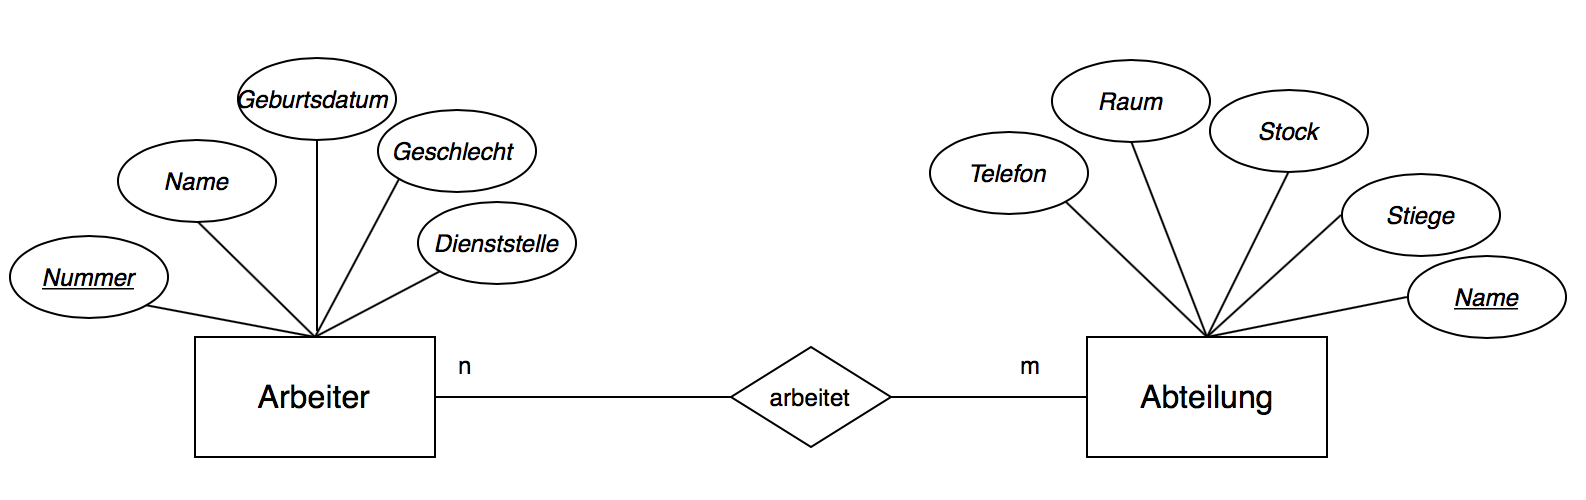
\includegraphics[width=0.7\textwidth]{images/ER.png}
\end{center}

Wie man auf der Diagramm sieht, Nummer ist der Schlüsselattribut beim Arbeiter, und Name ist Schlüsselattribut bei der Abteilung. Es liegt eine n:m Beziehung vor, weil ein Arbeiter kann in mehreren Abteilungen arbeiten, und eine Abteilung kann mehrere Arbeiter beinhalten. 
	In einem ER-Modell wird es zwischen 1:1, 1:n und n:m Beziehungen unterschieden, wie bei dem relationalen Datenmodell. In unserem Fall, ist es eine n:m Beziehung, weil mehrere Arbeiter können in mehreren Abteilungen arbeiten, und eine Abteilung kann mehrere Arbeiter beinhalten. Es gibt auch reflexive Beziehungen.
	Eine Erweiterung des Chen ER-Modells kann ein Konzept der Spezialisirung oder Generalisierung vorstellen, wobei es eine Abhängigkeit «Unterklasse-Oberkalsse» zwischen den Entitäten hergestellt wird. Oberklassen und Unterklassen werden dafür verwendet, dass eine Wiederholung von gemeinsamen Attributen vermieden wird. Die Unterklasse erbt alle Attribute und Abhängigkeiten der Oberklasse. 
	Man unterscheidet zwischen konzeptuellen und physischen ER-Modellen. Die konzeptuellen können die konkrete Eigenschaften einer Datenbank nicht völlig berücksichtigen, aber die physische werden nach der Regeln von Datenbank gebildet stellen ein Prototyp der Datenbank dar. Entitäten aus der ER-Diagramm werden zu den Tabellen, Attribute werden zur Spalten, wobei man die zulässige Datentypen und Namen von Spalten berücksichtigt. Die Beziehungen werden durch Migration der Schlüsselattributen von Eltern-Tabellen und Erzeugung von Fremdschlüsseln gebildet. Um die gegenseitige Abhängigkeit zwischen ER-Modell und relationalen Datenbankmodell zu zeigen, werden wir die wichtigsten Schritte einer Verwandlung von ER zum relatioanalen Modell angeben.
    
    
\begin{enumerate}
\item  Jede einfache Entität wird in eine Tabelle umgewandelt. Einfache Entität ist eine Entität, die keine Unter- bzw. Oberklassen hat.
\item  Jedes Attribut wird zu der möglichen Spalte mit dem entsprechenden Namen, und ein passendes Datentyp wird gewählt. Mehrwertige Attribute müssen zerlegt werden und Zusammengesetzte Attribute müssen als Neue Entitäten behandelt werden. 
\item  Die Schlüsselattribute werden zu dem Primary Keys der Tabelle. Wenn es mehrere Schlüsselattribute gibt, dann muss nur ein passendes ausgewählt werden. 
\item  Die n:m Beziehungen muss man als eigene Relationen dargestellen, mit den entsprechenden Primary und Foreign Schlüsseln , obwohl die 1:1 und 1:n muss man nicht als eine separate Tabelle machen, sondern nur in einer Relation, die in der Beziehung teilnimmt, entsprechendes Foreign Key angeben.
\end{enumerate}


Es ist eine große Anzahl von grafischen Notationen für die Darstellung von ER-Modellen bekannt. Zum Vorbild ist aber eine Notation geworden, die von Charles Bachmann im Jahr 1969 bereitgestellt wurde \cite{bachman1969data}, und für die Darstellung von Netzwerkmodell der Daten verwendet wurde. Der nächste Schritt wurde im Jahr 1975 von  Peter Chen, der eine neue Notation vorgeschlagen hat \cite{barker1990case}, für die Darstellung von Elementen nicht nur der konzeptuellen Ebene, sondern auch des logischen. In 1986 hat Richard Barker die Ideen von Chen und Bachmann verwendet und ein erfand seine eigene Notation, die dann als Grundlage für die weitere Entwicklungen diente. Für die Entwicklung von ER-Modellen wird spezielles Software benutzt, die sogenannte CASE-mittel, die in der Mitte von 1980 Jahren erschienen. Die Abkürzung CASE hat zwei Auslegungen: Computer-Aided Software Engineering (Entwicklung der Programme mit Hilfe von Computer) und Computer-Aided System Engineering. Heutzutage versteht man unter CASE-programme eine Menge von Instrumenten, die für die Entwicklung der strukturellen Teilen von Programmen, Systemen und Prozessen geeignet ist. Unter dieser Menge gibt es auch Mittel für die Entwicklung von ER-Modellen unter Verwendung von den populärsten Notationen: Chen-Notation, Barker-Notation, Bachmann Notation, usw. Die meistbenutzte  Werkzeuge sind CA Erwin Data Modeler (Hersteller - Computer Associates), Oracle Designer (Oracle Corporation), Power Designer (Sybase), MS Visio, usw. Die meisten Produkte unterstützen oft Barker- und Bachmann Notationen, aber selten Chen Notation. Alle Werkzeuge außer Visio (Microsoft) unterstützen eine Umwandlung des konzeptuelles Schemas in eine physische Beschreibungssprache SQL eines beliebigen Datenbanksystem. 

Der Fortschritt von konzeptuellen Darstellung der Daten geht immer weiter. Als Vorschlag für die Richtung der Weiterentwicklung des ER-Modells kann sein, dass es dem Benutzer ermöglicht wird, das konzeptuelles ER Modell zu korrigieren und ändern und die Datenbank wird alle Änderungen und Korrekturen automatisch berücksichtigen, und seine Struktur entsprechend ändern. 




%~ \hspace{1 cm}

%~ \newpage
%~ \bibliographystyle{plain}
%~ \bibliography{biblist}

%~ \end{document}
